% chktex-file 1

\FloatBarrier
\section{\large Ejercicio 3. Bases ortogonales de $\mathbb{R}^3$}

Determine si el conjunto \textbf{\textit{S}} corresponde a una base ortogonal de $\mathbb{R}^3$. En caso contrario, explique por qué no cumple con las condiciones de una base ortogonal.

\[
    \text{\textbf{\textit{S}}}=\left\{(-1,0,0),(0,-4,0),(0,0,5)\right\}
\]

\begin{itemize}
    \item \textit{Es un conjunto linealmente independiente.}
    \[
        \left|\text{\textbf{\textit{S}}}\right|=
        \begin{vmatrix}
            -1 & 0 & 0 \\
            0 & -4 & 0 \\
            0 & 0 & 5 \\
            -1 & 0 & 0 \\
            0 & -4 & 0 \\
        \end{vmatrix}
        =20
    \]
    \begin{center}
        \textbf{\textit{Si es un conjunto linealmente independiente porque el determinante es diferente de 0.}}
    \end{center}
    \item \textit{El producto escalar entre cualquier par de vectores distintos de la base es 
    cero, lo que implica que los vectores son perpendiculares entre sí.}
    \[
        \vec{v1}\cdot\vec{v2}=(-1,0,0)\cdot(0,-4,0)=0+0+0=0
    \]
    \[
        \vec{v1}\cdot\vec{v3}=(-1,0,0)\cdot(0,0,5)=0+0+0=0
    \]
    \[
        \vec{v2}\cdot\vec{c3}=(0,-4,0)\cdot(0,0,5)=0+0+0=0
    \]
    \begin{center}
        \textbf{\textit{Los vectores si son perpendiculares entre sí.}}
    \end{center}
    \item \textit{La base contiene el número máximo de vectores linealmente independientes 
    posible para el espacio vectorial dado.}
    \begin{center}
        \textbf{\textit{Dado a que estamos trabajando en un espacio $\mathbb{R}^3$, el conjunto está formado por 3 vectores $\mathbb{R}^3$ y además, el conjunto es linealmente independiente, entonces sí contiene el número máximo de vectores linealmente independientes posible para el espacio vectorial dado.}}
    \end{center}
\end{itemize}

\begin{figure}[ht!]
    \centering
    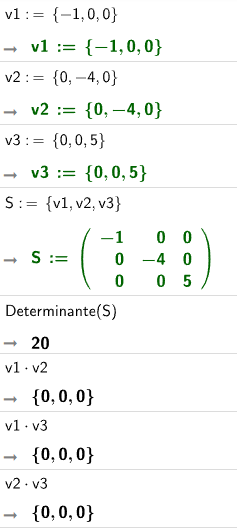
\includegraphics[width=150pt,height=250pt]{img/imagen11.png}
    \caption{Comprobación en GeoGebra}
\end{figure}
\textbf{Solución: }Teniendo en cuente que el conjunto \textbf{\textit{S}} cumple todas las condiciones anteriores entonces si se trata de una base ortogonal.